\paragraph{Мейн}
Бинарный файл (ELF, x86\_64), в котором пользователь должен \("\)угадывать\("\) случайные числа.
\begin{verbatim}
        undefined8 FUN_00101200(void)

        {
          undefined *__s;
          uint in_EAX;
          time_t tVar1;
          long lVar2;
          size_t sVar3;
          int iVar4;
          int iVar5;
          int iVar6;
          ulong uVar7;
          undefined8 uStack_28;

          uStack_28 = (ulong)in_EAX;
          puts("Hello, You have to predict random numbers:");
          tVar1 = time((time_t *)0x0);
          srandom((uint)tVar1);
          iVar6 = 0x539;
          iVar5 = 0;
          do {
             __isoc99_scanf(&DAT_0010202b,(long)&uStack_28 + 4);
             lVar2 = random();
             __s = PTR_DAT_00104068;
             iVar4 = iVar5 + (uint)(lVar2 % 2 == (long)uStack_28._4_4_) * 2;
             iVar5 = iVar4 + -1;
             iVar6 = iVar6 + -1;
          } while (iVar6 != 0);
          if (iVar5 == 0x539) {
             if (*PTR_DAT_00104068 != '\0') {
                uVar7 = 0;
                do {
                  putchar((int)(char)__s[uVar7] ^ iVar4 - 0x52dU);
                  uVar7 = uVar7 + 1;
                  sVar3 = strlen(__s);
                } while (uVar7 < sVar3);
             }
          }
          else {
             printf("Oh noo ...");
          }
          return 0;
        }
\end{verbatim}

\paragraph{Описание}
\begin{itemize}
    \item Бинарный файл выводит: \("\)Hello, You have to predict random numbers:\("\)
    Затем вызывает \texttt{srandom(time(NULL))}, делая генератор случайных чисел предсказуемым, если известен момент запуска.

    \item Цикл длин ой 1337 итераций, где:
    \item Генерируется случайное число \texttt{random()}.
    \item Пользователь вводит 0 или 1 (угадывает чётность).
    \item Если угадывает — увеличивается счётчик.
    \item После 1337 правильных угадываний сравнивается результат:
    \item Если все угадывания верны — расшифровывается строка \texttt{PTR\_DAT\_00104068} с помощью XOR .
    \item XOR ключ вычисляется как \texttt{(iVar4 - 0x52d) = 1338--1325 = 13}.
\end{itemize}

Используя команду \texttt{strings task\_4} я получил что-то похожее на заiифрованный ключ: \texttt{kaljv44o<kk5k<<:5<89<k:k54k4oi9<n9l<:p}

Я создал питоновский скрипт, который использует библиотеки \texttt{random} для симуляции рандомного поведения кода
подбора букв и \texttt{time} для использования сида.
Далее скрипт дешифровывает с XOR ключом искомый флаг.
Найти скрипт можно по ссылке\cite{githublink}

\paragraph{Особенности}
\begin{itemize}
    \item Задача построена на использовании random() из glibc, который инициализируется с помощью srandom(time(NULL)).
    \item Это предсказуемо, если у нас есть примерное время запуска программы.
    \item Зашифрованный ключ: \texttt{kaljv44o<kk5k<<:5<89<k:k54k4oi9<n9l<:p}
    \item Дешифрованный ключ: \texttt{flag\{99b1ff8f11781541f7f89f9bd41c4a17\}}
\end{itemize}

\paragraph{Тестовый запуск}
Аутпут питоновского скрипта:

\paragraph{}
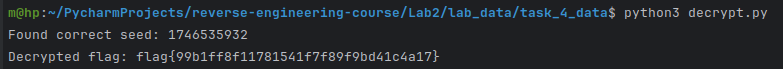
\includegraphics[width=1\linewidth]{static/solution_task_4}
